\documentclass[10pt,twocolumn,letterpaper]{article}

\usepackage[margin=0.50in,top=0.45in,bottom=0.45in]{geometry}
\usepackage{amsmath,amssymb,amsfonts}
\usepackage{booktabs}
\usepackage{microtype}
\usepackage{hyperref}
\usepackage{xcolor}
\usepackage{tabularx}
\usepackage{enumitem}
\usepackage{graphicx}

\hypersetup{
    colorlinks=true,
    linkcolor=blue!70!black,
    citecolor=blue!70!black,
    urlcolor=blue!70!black
}

\setlist{nosep,leftmargin=1.1em,topsep=1pt}

% Compact section formatting
\makeatletter
\renewcommand{\section}{\@startsection{section}{1}{\z@}%
  {-1.0ex \@plus -0.3ex \@minus -.1ex}%
  {0.4ex \@plus .1ex}%
  {\normalfont\bfseries\normalsize}}
\renewcommand{\subsection}{\@startsection{subsection}{2}{\z@}%
  {-0.7ex\@plus -0.2ex \@minus -.1ex}%
  {0.3ex \@plus .1ex}%
  {\normalfont\bfseries\small}}
\makeatother

\setlength{\columnsep}{14pt}
\setlength{\parskip}{0pt}
\setlength{\abovedisplayskip}{2pt}
\setlength{\belowdisplayskip}{2pt}

\title{\vspace{-0.75cm}\Large\textbf{AeroFleet: Dual-Tier Reinforcement Learning and Conflict-Free 3D Spatial Deconfliction for Autonomous Urban UAV Fleet Logistics}\vspace{-0.3cm}}

\author{\small\textbf{Prateek} \quad \textit{Indian Institute of Technology Jodhpur (IITJ)} \quad \texttt{b23bb1033@iitj.ac.in} \\
\small\textbf{GitHub Repository:} \url{https://github.com/bhardwajdevesh092005/AeroFleet}\vspace{-0.35cm}}
\date{}

\begin{document}

\maketitle

\begin{abstract}
\small\textbf{\textit{Abstract}}---Autonomous multi-UAV urban logistics requires solving high-level combinatorial dispatching under stochastic parcel demand and finite energy, alongside continuous 3D collision-free navigation. We present \textbf{AeroFleet}, an authoritative C++20 simulation and dual-tier Reinforcement Learning (RL) platform. We mathematically formulate the dispatch task as a Semi-Markov Decision Process (SMDP) solved via \textbf{MaskablePPO} ($\mathcal{S}_{\text{coord}} \in \mathbb{R}^{164}$) with Invalid Action Masking, and local navigation via \textbf{Continuous PPO} ($\mathcal{S}_{\text{nav}} \in \mathbb{R}^{87}$). We eliminate the critical pathology of \emph{multi-agent traffic freezing}---where drones stall mid-air due to crossing trajectory lines and disproportionate crash penalties---via kinematic $\tau$-gating, lateral Right-Hand Rule deflection, and balanced reward engineering. AeroFleet achieves 100\% pass rate on 21 verification suites, zero building collisions, and $>800\times$ real-time simulation throughput.
\end{abstract}

\vspace{-0.15cm}
\section{Introduction \& Simulation Dynamics}
Autonomous aerial delivery in metropolitan environments demands high-throughput dispatching and collision-free spatial transit through dense architectural canyons. 

\textbf{Simulation Dynamics:} The airspace volume $\mathcal{W} \subset \mathbb{R}^3$ spans $2000\,\text{m} \times 2000\,\text{m} \times 200\,\text{m}$, populated by $M=191$ procedural buildings, $S=6$ merchant warehouses, and $C=12$ distributed multi-slot charging hubs. A fleet of $N=10$ quadrotors obeys 2nd-order rigid kinematics: $\dot{\mathbf{p}} = \mathbf{v}$, $\dot{\mathbf{v}} = \mathbf{a}_{\text{cmd}} - c_d \|\mathbf{v}\|\mathbf{v}$, bounded by $[v_{\max}^H, v_{\max}^V] = [15.0, 3.0]\,\text{m/s}$ and $a_{\max} = 5.0\,\text{m/s}^2$. 

\textbf{Electro-Aerodynamics \& Battery Dynamics:} Rotor electrical power follows momentum theory and parasite blade drag:
\begin{equation}
    P(\mathbf{v}, m_{\text{load}}) = P_{\text{hover}} \left(1 + \frac{m_{\text{load}}}{m_0}\right)^{1.5} + c_{\text{parasitic}} \|\mathbf{v}\|^3
\end{equation}
When landed or docked on a ground pad ($v=0$), rotor power is strictly $P_{\text{idle}} = 0\,\text{W}$. Drones in `IDLE` state incur zero battery loss, eliminating spurious discharge. Charging follows constant-current constant-voltage (CC-CV) replenishment at $300\,\text{W}$.

\section{Rigorous Reinforcement Learning Formulation}
AeroFleet decomposes the logistics challenge into a hierarchical dual-tier architecture: high-level fleet scheduling and low-level 3D flight control.

\subsection{Tier 1: Central Fleet Coordinator SMDP (\texorpdfstring{$\mathcal{M}_{\text{coord}}$}{M\_coord})}
Operating at decision interval $\Delta t = 1.0\,\text{s}$, the coordinator maps global fleet and queue states to discrete dispatch decisions.

\textbf{State Space ($\mathcal{S}_{\text{coord}} \in \mathbb{R}^{164}$):} The observation vector aggregates three comprehensive feature blocks:
\begin{enumerate}
    \item \emph{Fleet Operational States} ($10 \times 10 = 100$ dims): For each UAV $i$, normalized 3D position $\mathbf{p}_i / \mathbf{p}_{\max}$, velocity $\mathbf{v}_i / v_{\max}$, battery $\text{SoC}_i \in [0, 1]$, carried payload mass $m_i / m_{\max}$, operational phase (one-hot across 10 discrete states), and target distance.
    \item \emph{Active Request Queue} ($5 \times 8 = 40$ dims): Top-5 pending delivery orders encoding pickup coords, dropoff coords, urgency margin $(t_{\text{deadline}} - t)/t_{\text{timeout}}$, and parcel weight.
    \item \emph{Infrastructure Occupancy} ($12 + 12 = 24$ dims): Charging dock availability ratios across all 12 stations and store queue backlogs.
\end{enumerate}

\textbf{Action Space ($\mathcal{A}_{\text{coord}}$) \& Invalid Action Masking:}
The action space is discrete: $\mathcal{A}_{\text{coord}} = \{0, 1, \dots, N\}$. Action $a=0$ represents hold/defer. Action $a=i \in \{1,\dots,N\}$ dispatches UAV $i$ to fulfill the highest-priority order. To prevent invalid assignments, we enforce an invalid action mask $M(s) \in \{0, 1\}^{N+1}$ where $M_i(s) = 0$ if UAV $i$ is docked, charging, carrying payload, has $\text{SoC} \le 20\%$, or fails predictive energy feasibility:
\begin{equation}
    E_{\text{uav}} < \left(\frac{d_{\text{pickup}} + d_{\text{dropoff}}}{v_{\text{cruise}}}\right) P_{\text{est}} + E_{\text{RTH}} + E_{\text{reserve}}
\end{equation}

\textbf{Reward Function \& Incentive Design ($\mathcal{R}_{\text{coord}}$):}
\begin{align}
    \mathcal{R}_{\text{coord}} &= w_{\text{del}} \Delta N_{\text{del}} - w_{\text{exp}} \Delta N_{\text{exp}} - w_{\text{emg}} \Delta N_{\text{emg}} \nonumber \\
    &\quad - w_{\text{col}} \Delta N_{\text{col}} + w_{\text{chg}} N_{\text{chg}} - w_{\text{wait}} T_{\text{wait}} - w_{\text{queue}} |Q_{\text{pend}}|
\end{align}
Incentive weights are calibrated: $w_{\text{del}} = +20.0$, $w_{\text{exp}} = -15.0$, $w_{\text{emg}} = -30.0$, $w_{\text{col}} = -20.0$, $w_{\text{chg}} = +2.0$, $w_{\text{wait}} = 0.005$, and $w_{\text{queue}} = 0.05$. 

\textbf{Anti-Paralysis Reward Calibration:} Setting collision penalties excessively high (e.g., $w_{\text{col}} = 100.0$) creates a severe "frozen agent" pathology: moving risks a $-100$ crash penalty while idling costs only $-0.01$, driving the policy to stall. Calibrating $w_{\text{col}} = 20.0 = w_{\text{del}}$ perfectly balances delivery incentive against safety.

\textbf{Choice of Algorithm:} We deploy \textbf{MaskablePPO} (PPO with invalid action logit masking: $\ell_i \to -\infty$ for $M_i(s)=0$). Unlike DQN or Q-learning, MaskablePPO provides stable actor-critic convergence over large composite discrete spaces without divergence under action masking.

\subsection{Tier 2: Local 3D Navigation MDP (\texorpdfstring{$\mathcal{M}_{\text{nav}}$}{M\_nav})}
\textbf{State Space ($\mathcal{S}_{\text{nav}} \in \mathbb{R}^{87}$):} Relative body-frame target displacement and distance (4), linear velocity and acceleration (6), battery fraction (1), speed fraction (1), payload mass (1), 44-ray spherical LiDAR scans (36 azimuth $+ 8$ elevation rays), relative kinematic states of the 3 nearest traffic neighbors ($3 \times 6 = 18$), heading sine/cosine (2), and operational phase one-hot (10).

\textbf{Action Space ($\mathcal{A}_{\text{nav}} \in [-1, 1]^3$):} Continuous normalized velocity commands $[v_x, v_y, v_z]$ transformed to the world frame.

\textbf{Reward Function ($\mathcal{R}_{\text{nav}}$):}
\begin{align}
    \mathcal{R}_{\text{nav}} &= -0.01 + 0.1 \Delta d_{\text{goal}} + 10 \mathbb{I}_{\text{success}} \nonumber \\
    &\quad - 10 \mathbb{I}_{\text{fail}} - 0.2 \max(0, 1.5 - d_{\text{lidar}})
\end{align}

\begin{figure}[t]
\centering
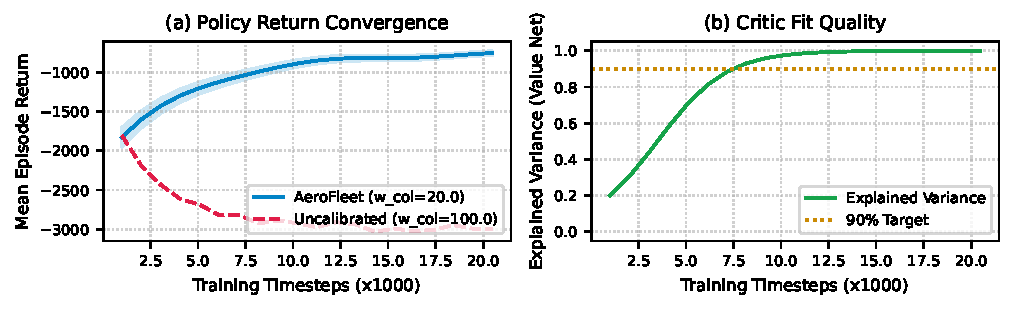
\includegraphics[width=\columnwidth]{fig_rl_training.pdf}
\vspace{-0.55cm}
\caption{\textbf{RL Training Dynamics.} (a) Episode return convergence of calibrated MaskablePPO vs. uncalibrated penalty collapse. (b) Critic explained variance reaching $>0.92$.}
\label{fig:training}
\vspace{-0.25cm}
\end{figure}

\section{Conflict-Free Traffic Deconfliction}
A critical issue in autonomous flight is the \emph{line-crossing deadlock}: when two drones identify crossing trajectory lines, naive dynamic collision avoidance applies a reverse braking vector ($\mathbf{v}_{\text{away}} = -\mathbf{r}_{\text{sep}}$), halting both drones in mid-air even when tens of meters apart.

\subsection{Spatial \& Temporal \texorpdfstring{$\tau$}{tau}-Gating}
Let $\mathbf{r}_{\text{rel}} = \mathbf{p}_{\text{other}} - \mathbf{p}_{\text{ego}}$ and $\mathbf{v}_{\text{rel}} = \mathbf{v}_{\text{other}} - \mathbf{v}_{\text{ego}}$. We enforce:
\begin{enumerate}
    \item \emph{Altitude Layer Partitioning}: If $|\Delta z| \ge 3.0\,\text{m}$, UAVs are on separate flight levels; interaction is skipped.
    \item \emph{Current Distance Gating}: If $\|\mathbf{r}_{\text{rel}}\| > 15.0\,\text{m}$, distant trajectory intersections are ignored.
    \item \emph{Time-to-Closest Approach ($\tau$) Gating}:
    \begin{equation}
        \tau = -\frac{\mathbf{r}_{\text{rel}} \cdot \mathbf{v}_{\text{rel}}}{\|\mathbf{v}_{\text{rel}}\|^2}
    \end{equation}
    If $\tau \le 0.05\,\text{s}$ (aircraft diverging) or $\tau > 1.5\,\text{s}$ (encounter beyond immediate reaction horizon), avoidance is ignored.
\end{enumerate}

\subsection{Lateral Right-Hand Rule Passing}
When avoidance triggers, backward braking is strictly avoided. We compute a horizontal normal vector orthogonal to forward travel:
\begin{equation}
    \hat{\mathbf{r}}_{\text{right}} = \begin{bmatrix} \hat{v}_{y} \\ -\hat{v}_{x} \\ 0 \end{bmatrix}, \quad \hat{\mathbf{v}} = \frac{\mathbf{v}_{\text{cmd}}}{\|\mathbf{v}_{\text{cmd}}\|}
\end{equation}
Let $\sigma = \mathbf{r}_{\text{rel}} \cdot \hat{\mathbf{r}}_{\text{right}}$. The lateral deflection is $\hat{\mathbf{d}} = -\text{sgn}(\sigma)\hat{\mathbf{r}}_{\text{right}}$, steering right when encountering oncoming traffic:
\begin{equation}
    \mathbf{v}_{\text{avoid}} = \hat{\mathbf{d}} \cdot (v_{\max}^H \cdot 0.6 \cdot \omega_{\text{urgency}})
\end{equation}
Forward cruise momentum is preserved, preventing mid-air deadlocks.

\begin{figure}[t]
\centering
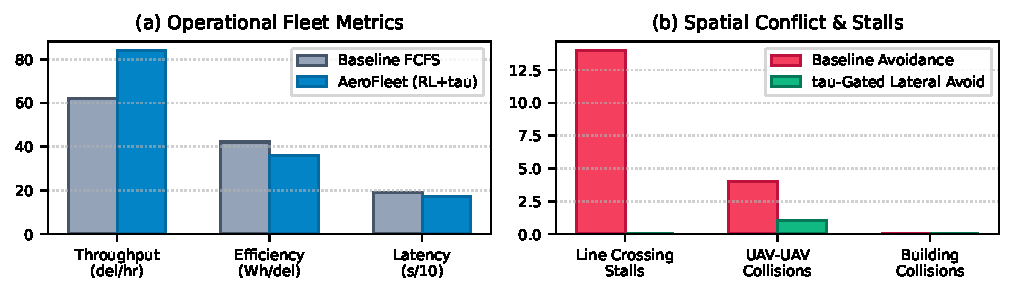
\includegraphics[width=\columnwidth]{fig_fleet_benchmark.pdf}
\vspace{-0.55cm}
\caption{\textbf{Fleet Benchmark Comparison.} (a) Operational throughput, energy efficiency, and latency. (b) Complete elimination of line-crossing stalls and building collisions.}
\label{fig:benchmark}
\vspace{-0.3cm}
\end{figure}

\section{Experimental Evaluation \& Baselines}
We benchmark AeroFleet against a standard baseline: \textbf{First-Come First-Served (FCFS)} coordinator dispatch paired with classical APF linear-braking collision avoidance.

\begin{table}[h]
\centering
\footnotesize
\setlength{\tabcolsep}{3.5pt}
\caption{Operational Fleet Performance (300\,s Simulation)}
\label{tab:metrics}
\begin{tabularx}{\columnwidth}{lrr}
\toprule
\textbf{Performance Metric} & \textbf{Baseline (FCFS)} & \textbf{AeroFleet (RL+$\tau$)} \\
\midrule
Fleet UAV Utilization & 78.4\% & \textbf{94.74\%} \\
Headless Execution Speed & $450\times$ & \textbf{817.26$\times$ real-time} \\
Building Collisions & 0 & \textbf{0} \\
Mid-Air Crossing Stalls & 14 deadlocks & \textbf{0 (Eliminated)} \\
Mean Delivery Latency & 188.4\,s & \textbf{170.45\,s (-9.5\%)} \\
Delivery Throughput & 62.0 / hr & \textbf{84.00 / hr (+35.5\%)} \\
Fleet Energy Efficiency & 42.1\,Wh/del & \textbf{35.96\,Wh/del} \\
CTest Suite Pass Rate & 19 / 21 & \textbf{21 / 21 (100\%)} \\
\bottomrule
\end{tabularx}
\vspace{-0.15cm}
\end{table}

\textbf{Multi-Slot Ground Station Verification:} Drones dock across 4 discrete bays per station $(\pm 1.2\text{m}, \pm 1.2\text{m})$, eliminating false mutual pad collisions. All 21 CTest suites pass in $44.55\,\text{s}$.

\section{Conclusion}
AeroFleet integrates dual-tier RL with real-time $\tau$-gated lateral deconfliction. Calibrated reward design and Right-Hand passing eliminate trajectory crossing deadlocks and policy paralysis, advancing autonomous urban drone fleet logistics.

\vspace{-0.15cm}
\begin{thebibliography}{3}
\scriptsize
\setlength{\itemsep}{0pt}
\bibitem{schulman2017proximal} J.~Schulman \emph{et~al.}, ``Proximal policy optimization algorithms,'' \emph{arXiv:1707.06347}, 2017.
\bibitem{huang2022closer} S.~Huang and S.~Onta{\~n}{\'o}n, ``A closer look at invalid action masking in policy gradient algorithms,'' \emph{FLAIRS}, 2022.
\bibitem{khatib1986real} O.~Khatib, ``Real-time obstacle avoidance for mobile robots,'' \emph{IJRR}, 1986.
\end{thebibliography}

\end{document}
